% Options for packages loaded elsewhere
\PassOptionsToPackage{unicode}{hyperref}
\PassOptionsToPackage{hyphens}{url}
%
\documentclass[
  11pt,
]{article}
\usepackage{amsmath,amssymb}
\usepackage{lmodern}
\usepackage{iftex}
\ifPDFTeX
  \usepackage[T1]{fontenc}
  \usepackage[utf8]{inputenc}
  \usepackage{textcomp} % provide euro and other symbols
\else % if luatex or xetex
  \usepackage{unicode-math}
  \defaultfontfeatures{Scale=MatchLowercase}
  \defaultfontfeatures[\rmfamily]{Ligatures=TeX,Scale=1}
\fi
% Use upquote if available, for straight quotes in verbatim environments
\IfFileExists{upquote.sty}{\usepackage{upquote}}{}
\IfFileExists{microtype.sty}{% use microtype if available
  \usepackage[]{microtype}
  \UseMicrotypeSet[protrusion]{basicmath} % disable protrusion for tt fonts
}{}
\makeatletter
\@ifundefined{KOMAClassName}{% if non-KOMA class
  \IfFileExists{parskip.sty}{%
    \usepackage{parskip}
  }{% else
    \setlength{\parindent}{0pt}
    \setlength{\parskip}{6pt plus 2pt minus 1pt}}
}{% if KOMA class
  \KOMAoptions{parskip=half}}
\makeatother
\usepackage{xcolor}
\IfFileExists{xurl.sty}{\usepackage{xurl}}{} % add URL line breaks if available
\IfFileExists{bookmark.sty}{\usepackage{bookmark}}{\usepackage{hyperref}}
\hypersetup{
  pdftitle={SURVIVAL ANALYSIS - NCDB},
  pdfauthor={Kelvin Ofori-Minta; University of Texas at El Paso (UTEP)},
  hidelinks,
  pdfcreator={LaTeX via pandoc}}
\urlstyle{same} % disable monospaced font for URLs
\usepackage[margin=1in]{geometry}
\usepackage{color}
\usepackage{fancyvrb}
\newcommand{\VerbBar}{|}
\newcommand{\VERB}{\Verb[commandchars=\\\{\}]}
\DefineVerbatimEnvironment{Highlighting}{Verbatim}{commandchars=\\\{\}}
% Add ',fontsize=\small' for more characters per line
\usepackage{framed}
\definecolor{shadecolor}{RGB}{248,248,248}
\newenvironment{Shaded}{\begin{snugshade}}{\end{snugshade}}
\newcommand{\AlertTok}[1]{\textcolor[rgb]{0.94,0.16,0.16}{#1}}
\newcommand{\AnnotationTok}[1]{\textcolor[rgb]{0.56,0.35,0.01}{\textbf{\textit{#1}}}}
\newcommand{\AttributeTok}[1]{\textcolor[rgb]{0.77,0.63,0.00}{#1}}
\newcommand{\BaseNTok}[1]{\textcolor[rgb]{0.00,0.00,0.81}{#1}}
\newcommand{\BuiltInTok}[1]{#1}
\newcommand{\CharTok}[1]{\textcolor[rgb]{0.31,0.60,0.02}{#1}}
\newcommand{\CommentTok}[1]{\textcolor[rgb]{0.56,0.35,0.01}{\textit{#1}}}
\newcommand{\CommentVarTok}[1]{\textcolor[rgb]{0.56,0.35,0.01}{\textbf{\textit{#1}}}}
\newcommand{\ConstantTok}[1]{\textcolor[rgb]{0.00,0.00,0.00}{#1}}
\newcommand{\ControlFlowTok}[1]{\textcolor[rgb]{0.13,0.29,0.53}{\textbf{#1}}}
\newcommand{\DataTypeTok}[1]{\textcolor[rgb]{0.13,0.29,0.53}{#1}}
\newcommand{\DecValTok}[1]{\textcolor[rgb]{0.00,0.00,0.81}{#1}}
\newcommand{\DocumentationTok}[1]{\textcolor[rgb]{0.56,0.35,0.01}{\textbf{\textit{#1}}}}
\newcommand{\ErrorTok}[1]{\textcolor[rgb]{0.64,0.00,0.00}{\textbf{#1}}}
\newcommand{\ExtensionTok}[1]{#1}
\newcommand{\FloatTok}[1]{\textcolor[rgb]{0.00,0.00,0.81}{#1}}
\newcommand{\FunctionTok}[1]{\textcolor[rgb]{0.00,0.00,0.00}{#1}}
\newcommand{\ImportTok}[1]{#1}
\newcommand{\InformationTok}[1]{\textcolor[rgb]{0.56,0.35,0.01}{\textbf{\textit{#1}}}}
\newcommand{\KeywordTok}[1]{\textcolor[rgb]{0.13,0.29,0.53}{\textbf{#1}}}
\newcommand{\NormalTok}[1]{#1}
\newcommand{\OperatorTok}[1]{\textcolor[rgb]{0.81,0.36,0.00}{\textbf{#1}}}
\newcommand{\OtherTok}[1]{\textcolor[rgb]{0.56,0.35,0.01}{#1}}
\newcommand{\PreprocessorTok}[1]{\textcolor[rgb]{0.56,0.35,0.01}{\textit{#1}}}
\newcommand{\RegionMarkerTok}[1]{#1}
\newcommand{\SpecialCharTok}[1]{\textcolor[rgb]{0.00,0.00,0.00}{#1}}
\newcommand{\SpecialStringTok}[1]{\textcolor[rgb]{0.31,0.60,0.02}{#1}}
\newcommand{\StringTok}[1]{\textcolor[rgb]{0.31,0.60,0.02}{#1}}
\newcommand{\VariableTok}[1]{\textcolor[rgb]{0.00,0.00,0.00}{#1}}
\newcommand{\VerbatimStringTok}[1]{\textcolor[rgb]{0.31,0.60,0.02}{#1}}
\newcommand{\WarningTok}[1]{\textcolor[rgb]{0.56,0.35,0.01}{\textbf{\textit{#1}}}}
\usepackage{graphicx}
\makeatletter
\def\maxwidth{\ifdim\Gin@nat@width>\linewidth\linewidth\else\Gin@nat@width\fi}
\def\maxheight{\ifdim\Gin@nat@height>\textheight\textheight\else\Gin@nat@height\fi}
\makeatother
% Scale images if necessary, so that they will not overflow the page
% margins by default, and it is still possible to overwrite the defaults
% using explicit options in \includegraphics[width, height, ...]{}
\setkeys{Gin}{width=\maxwidth,height=\maxheight,keepaspectratio}
% Set default figure placement to htbp
\makeatletter
\def\fps@figure{htbp}
\makeatother
\setlength{\emergencystretch}{3em} % prevent overfull lines
\providecommand{\tightlist}{%
  \setlength{\itemsep}{0pt}\setlength{\parskip}{0pt}}
\setcounter{secnumdepth}{5}
\usepackage{amsmath}
\usepackage{amssymb, bm}
\usepackage{amsfonts}
\usepackage{amsthm}
\usepackage{fancyhdr}
\pagestyle{fancy}
\fancyhf{}
\rhead{Summer RA}
\lhead{NCDB Research}
\cfoot{\thepage}
\usepackage{algorithm}
\usepackage[noend]{algpseudocode}
\usepackage{booktabs}
\usepackage{longtable}
\usepackage{array}
\usepackage{multirow}
\usepackage{wrapfig}
\usepackage{float}
\usepackage{colortbl}
\usepackage{pdflscape}
\usepackage{tabu}
\usepackage{threeparttable}
\usepackage{threeparttablex}
\usepackage[normalem]{ulem}
\usepackage{makecell}
\usepackage{xcolor}
\ifLuaTeX
  \usepackage{selnolig}  % disable illegal ligatures
\fi

\title{SURVIVAL ANALYSIS - NCDB}
\author{Kelvin Ofori-Minta \and University of Texas at El Paso (UTEP)}
\date{July 05, 2022}

\begin{document}
\maketitle

{
\setcounter{tocdepth}{4}
\tableofcontents
}
\newpage
\section{Loading Data and Preparations}

\begin{Shaded}
\begin{Highlighting}[]
\NormalTok{lung}\OtherTok{\textless{}{-}}\FunctionTok{read.csv}\NormalTok{(}\StringTok{"lung\_data2.csv"}\NormalTok{) }\CommentTok{\#predictors of mortality}
\end{Highlighting}
\end{Shaded}

\subsection{Partition Data}

\begin{Shaded}
\begin{Highlighting}[]
\FunctionTok{require}\NormalTok{(caTools)}
\FunctionTok{set.seed}\NormalTok{(}\DecValTok{1}\NormalTok{)}
\NormalTok{split }\OtherTok{=} \FunctionTok{sample.split}\NormalTok{(lung}\SpecialCharTok{$}\NormalTok{DX\_LASTCONTACT\_DEATH\_MONTHS,}\AttributeTok{SplitRatio =} \FloatTok{0.85}\NormalTok{)}
\NormalTok{train}\OtherTok{=}\FunctionTok{subset}\NormalTok{(lung, split}\SpecialCharTok{==}\NormalTok{T)}
\NormalTok{test}\OtherTok{=}\FunctionTok{subset}\NormalTok{(lung, split}\SpecialCharTok{==}\NormalTok{F)}
\end{Highlighting}
\end{Shaded}

\newpage
\section{COXPH model for predictors of mortality - ALL DATA}

\begin{Shaded}
\begin{Highlighting}[]
\FunctionTok{library}\NormalTok{(}\StringTok{"survival"}\NormalTok{)}
\CommentTok{\# library("survminer")}

\NormalTok{lung}\SpecialCharTok{$}\NormalTok{Chemo}\OtherTok{=}\FunctionTok{relevel}\NormalTok{(}\FunctionTok{as.factor}\NormalTok{(lung}\SpecialCharTok{$}\NormalTok{Chemo), }\AttributeTok{ref=}\StringTok{"No Chemo"}\NormalTok{)}
\NormalTok{cox\_fit1 }\OtherTok{\textless{}{-}} \FunctionTok{coxph}\NormalTok{(}\FunctionTok{Surv}\NormalTok{(DX\_LASTCONTACT\_DEATH\_MONTHS,PUF\_VITAL\_STATUS) }\SpecialCharTok{\textasciitilde{}}\NormalTok{ Chemo }\SpecialCharTok{+}
\NormalTok{                      AGE\_cat}\SpecialCharTok{+}       
\NormalTok{                      SEX }\SpecialCharTok{+}                     
\NormalTok{                      CDCC\_TOTAL\_BEST  }\SpecialCharTok{+}         
\NormalTok{                      TUMOR\_SIZE\_cat  }\SpecialCharTok{+}          
\NormalTok{                      GRADE  }\SpecialCharTok{+}                 
\NormalTok{                      Visceral\_Pleural\_Invasion}\SpecialCharTok{+} 
\NormalTok{                      LYMPH\_VASCULAR\_INVASION2}\SpecialCharTok{+}  
\NormalTok{                      Margins  }\SpecialCharTok{+}                
\NormalTok{                      Lymph\_Nodes\_Sampled }\SpecialCharTok{+}    
\NormalTok{                      Excision\_less\_than1, }
                    \AttributeTok{data =}\NormalTok{ lung)}

\NormalTok{cox\_fit1}\SpecialCharTok{$}\NormalTok{coefficients }\CommentTok{\#odds}
\end{Highlighting}
\end{Shaded}

\begin{verbatim}
##                       ChemoChemo                     AGE_cat60-70 
##                    -0.0328323599                    -0.0427297280 
##                     AGE_cat70-80                  AGE_catAbove 80 
##                    -0.0325108982                    -0.0430062924 
##                  AGE_catBelow 50                          SEXMale 
##                    -0.0909712523                    -0.0510721635 
##                 CDCC_TOTAL_BEST1                 CDCC_TOTAL_BEST2 
##                    -0.0021252500                    -0.0085577321 
##                 CDCC_TOTAL_BEST3            TUMOR_SIZE_cat1cm-2cm 
##                     0.0285513604                    -0.0839515534 
##            TUMOR_SIZE_cat2cm-3cm            TUMOR_SIZE_cat3cm-4cm 
##                    -0.1181348822                    -0.0801962360 
##            TUMOR_SIZE_cat4cm-5cm       GRADEPoorly differentiated 
##                    -0.0791002404                    -0.0002581338 
##            GRADEUndifferentiated                     GRADEUnknown 
##                     0.0907022956                     0.0039056293 
##         GRADEWell differentiated Visceral_Pleural_InvasionPresent 
##                    -0.0500901193                     0.0572583599 
##  LYMPH_VASCULAR_INVASION2Present  LYMPH_VASCULAR_INVASION2Unknown 
##                    -0.0234197701                    -0.1408796161 
##                  MarginsPositive                      MarginsZero 
##                     0.0570926793                     0.1810093997 
##          Lymph_Nodes_Sampled>=10       Lymph_Nodes_SampledUnknown 
##                     0.0522284067                    -0.2228574697 
##          Excision_less_than1TRUE 
##                    -0.0199985495
\end{verbatim}

\begin{Shaded}
\begin{Highlighting}[]
\FunctionTok{exp}\NormalTok{(cox\_fit1}\SpecialCharTok{$}\NormalTok{coefficients) }\CommentTok{\#HR}
\end{Highlighting}
\end{Shaded}

\begin{verbatim}
##                       ChemoChemo                     AGE_cat60-70 
##                        0.9677008                        0.9581703 
##                     AGE_cat70-80                  AGE_catAbove 80 
##                        0.9680119                        0.9579054 
##                  AGE_catBelow 50                          SEXMale 
##                        0.9130440                        0.9502101 
##                 CDCC_TOTAL_BEST1                 CDCC_TOTAL_BEST2 
##                        0.9978770                        0.9914788 
##                 CDCC_TOTAL_BEST3            TUMOR_SIZE_cat1cm-2cm 
##                        1.0289629                        0.9194758 
##            TUMOR_SIZE_cat2cm-3cm            TUMOR_SIZE_cat3cm-4cm 
##                        0.8885762                        0.9229352 
##            TUMOR_SIZE_cat4cm-5cm       GRADEPoorly differentiated 
##                        0.9239473                        0.9997419 
##            GRADEUndifferentiated                     GRADEUnknown 
##                        1.0949430                        1.0039133 
##         GRADEWell differentiated Visceral_Pleural_InvasionPresent 
##                        0.9511437                        1.0589294 
##  LYMPH_VASCULAR_INVASION2Present  LYMPH_VASCULAR_INVASION2Unknown 
##                        0.9768523                        0.8685939 
##                  MarginsPositive                      MarginsZero 
##                        1.0587539                        1.1984264 
##          Lymph_Nodes_Sampled>=10       Lymph_Nodes_SampledUnknown 
##                        1.0536164                        0.8002289 
##          Excision_less_than1TRUE 
##                        0.9802001
\end{verbatim}

\begin{Shaded}
\begin{Highlighting}[]
\CommentTok{\# lung$Chemo=relevel(as.factor(lung$Chemo), ref="No Chemo")}
\CommentTok{\# cox\_fit11 \textless{}{-} coxph(Surv(DX\_LASTCONTACT\_DEATH\_MONTHS,PUF\_VITAL\_STATUS) \textasciitilde{}}
\CommentTok{\#                       AGE\_cat+       }
\CommentTok{\#                       SEX +                     }
\CommentTok{\#                       CDCC\_TOTAL\_BEST  +         }
\CommentTok{\#                       TUMOR\_SIZE\_cat  +          }
\CommentTok{\#                       GRADE  +                 }
\CommentTok{\#                       Visceral\_Pleural\_Invasion+ }
\CommentTok{\#                       LYMPH\_VASCULAR\_INVASION2+  }
\CommentTok{\#                       Margins  +                }
\CommentTok{\#                       Lymph\_Nodes\_Sampled +    }
\CommentTok{\#                       Excision\_less\_than1, }
\CommentTok{\#                     data = lung)}
\CommentTok{\# }
\CommentTok{\# cox\_fit11$coefficients \#odds}
\CommentTok{\# }
\CommentTok{\# exp(cox\_fit11$coefficients) \#HR}
\end{Highlighting}
\end{Shaded}

\newpage

\hypertarget{format-results-of-cox-model}{%
\section{format results of cox
model}\label{format-results-of-cox-model}}

\begin{Shaded}
\begin{Highlighting}[]
\FunctionTok{require}\NormalTok{(kableExtra)}
\NormalTok{broom}\SpecialCharTok{::}\FunctionTok{tidy}\NormalTok{(cox\_fit1 , }
            \AttributeTok{exp=}\ConstantTok{TRUE}\NormalTok{) }\SpecialCharTok{\%\textgreater{}\%}
  \FunctionTok{kable}\NormalTok{()}
\end{Highlighting}
\end{Shaded}

\begin{tabular}{l|r|r|r|r}
\hline
term & estimate & std.error & statistic & p.value\\
\hline
ChemoChemo & 0.9677008 & 0.0296857 & -1.1059996 & 0.2687267\\
\hline
AGE\_cat60-70 & 0.9581703 & 0.0312769 & -1.3661761 & 0.1718837\\
\hline
AGE\_cat70-80 & 0.9680119 & 0.0316406 & -1.0275044 & 0.3041830\\
\hline
AGE\_catAbove 80 & 0.9579054 & 0.0464372 & -0.9261165 & 0.3543854\\
\hline
AGE\_catBelow 50 & 0.9130440 & 0.0736842 & -1.2346094 & 0.2169759\\
\hline
SEXMale & 0.9502101 & 0.0218628 & -2.3360333 & 0.0194895\\
\hline
CDCC\_TOTAL\_BEST1 & 0.9978770 & 0.0255017 & -0.0833377 & 0.9335830\\
\hline
CDCC\_TOTAL\_BEST2 & 0.9914788 & 0.0361173 & -0.2369425 & 0.8127014\\
\hline
CDCC\_TOTAL\_BEST3 & 1.0289629 & 0.0424419 & 0.6727165 & 0.5011277\\
\hline
TUMOR\_SIZE\_cat1cm-2cm & 0.9194758 & 0.0911452 & -0.9210746 & 0.3570115\\
\hline
TUMOR\_SIZE\_cat2cm-3cm & 0.8885762 & 0.0919570 & -1.2846749 & 0.1989059\\
\hline
TUMOR\_SIZE\_cat3cm-4cm & 0.9229352 & 0.0937552 & -0.8553788 & 0.3923415\\
\hline
TUMOR\_SIZE\_cat4cm-5cm & 0.9239473 & 0.0952241 & -0.8306742 & 0.4061577\\
\hline
GRADEPoorly differentiated & 0.9997419 & 0.0252995 & -0.0102031 & 0.9918592\\
\hline
GRADEUndifferentiated & 1.0949430 & 0.1025368 & 0.8845825 & 0.3763818\\
\hline
GRADEUnknown & 1.0039133 & 0.0381754 & 0.1023075 & 0.9185126\\
\hline
GRADEWell differentiated & 0.9511437 & 0.0339343 & -1.4760914 & 0.1399194\\
\hline
Visceral\_Pleural\_InvasionPresent & 1.0589294 & 0.0362535 & 1.5793890 & 0.1142468\\
\hline
LYMPH\_VASCULAR\_INVASION2Present & 0.9768523 & 0.0300965 & -0.7781551 & 0.4364776\\
\hline
LYMPH\_VASCULAR\_INVASION2Unknown & 0.8685939 & 0.0465820 & -3.0243343 & 0.0024918\\
\hline
MarginsPositive & 1.0587539 & 0.1968533 & 0.2900265 & 0.7717959\\
\hline
MarginsZero & 1.1984264 & 0.1782101 & 1.0157079 & 0.3097685\\
\hline
Lymph\_Nodes\_Sampled>=10 & 1.0536164 & 0.0224537 & 2.3260485 & 0.0200160\\
\hline
Lymph\_Nodes\_SampledUnknown & 0.8002289 & 0.0590297 & -3.7753459 & 0.0001598\\
\hline
Excision\_less\_than1TRUE & 0.9802001 & 0.0344942 & -0.5797649 & 0.5620732\\
\hline
\end{tabular}

\newpage

\begin{Shaded}
\begin{Highlighting}[]
\NormalTok{cox\_fit1 }\SpecialCharTok{\%\textgreater{}\%}
\NormalTok{  gtsummary}\SpecialCharTok{::}\FunctionTok{tbl\_regression}\NormalTok{(}\AttributeTok{exp=}\ConstantTok{TRUE}\NormalTok{)}
\end{Highlighting}
\end{Shaded}

\begin{tabular}{l|c|c|c}
\hline
**Characteristic** & **HR** & **95\% CI** & **p-value**\\
\hline
Chemo &  &  & \\
\hline
No Chemo &  &  & \\
\hline
Chemo & 0.97 & 0.91, 1.03 & 0.3\\
\hline
AGE\_cat &  &  & \\
\hline
50-60 &  &  & \\
\hline
60-70 & 0.96 & 0.90, 1.02 & 0.2\\
\hline
70-80 & 0.97 & 0.91, 1.03 & 0.3\\
\hline
Above 80 & 0.96 & 0.87, 1.05 & 0.4\\
\hline
Below 50 & 0.91 & 0.79, 1.05 & 0.2\\
\hline
SEX &  &  & \\
\hline
Female &  &  & \\
\hline
Male & 0.95 & 0.91, 0.99 & 0.019\\
\hline
CDCC\_TOTAL\_BEST &  &  & \\
\hline
0 &  &  & \\
\hline
1 & 1.00 & 0.95, 1.05 & >0.9\\
\hline
2 & 0.99 & 0.92, 1.06 & 0.8\\
\hline
3 & 1.03 & 0.95, 1.12 & 0.5\\
\hline
TUMOR\_SIZE\_cat &  &  & \\
\hline
<=1cm &  &  & \\
\hline
1cm-2cm & 0.92 & 0.77, 1.10 & 0.4\\
\hline
2cm-3cm & 0.89 & 0.74, 1.06 & 0.2\\
\hline
3cm-4cm & 0.92 & 0.77, 1.11 & 0.4\\
\hline
4cm-5cm & 0.92 & 0.77, 1.11 & 0.4\\
\hline
GRADE &  &  & \\
\hline
Moderately differentiated &  &  & \\
\hline
Poorly differentiated & 1.00 & 0.95, 1.05 & >0.9\\
\hline
Undifferentiated & 1.09 & 0.90, 1.34 & 0.4\\
\hline
Unknown & 1.00 & 0.93, 1.08 & >0.9\\
\hline
Well differentiated & 0.95 & 0.89, 1.02 & 0.14\\
\hline
Visceral\_Pleural\_Invasion &  &  & \\
\hline
Other &  &  & \\
\hline
Present & 1.06 & 0.99, 1.14 & 0.11\\
\hline
LYMPH\_VASCULAR\_INVASION2 &  &  & \\
\hline
Absent &  &  & \\
\hline
Present & 0.98 & 0.92, 1.04 & 0.4\\
\hline
Unknown & 0.87 & 0.79, 0.95 & 0.002\\
\hline
Margins &  &  & \\
\hline
Other &  &  & \\
\hline
Positive & 1.06 & 0.72, 1.56 & 0.8\\
\hline
Zero & 1.20 & 0.85, 1.70 & 0.3\\
\hline
Lymph\_Nodes\_Sampled &  &  & \\
\hline
<10 &  &  & \\
\hline
>=10 & 1.05 & 1.01, 1.10 & 0.020\\
\hline
Unknown & 0.80 & 0.71, 0.90 & <0.001\\
\hline
Excision\_less\_than1 &  &  & \\
\hline
FALSE &  &  & \\
\hline
TRUE & 0.98 & 0.92, 1.05 & 0.6\\
\hline
\end{tabular}

\newpage
\section{Predicting Risks scores and Hazard Ratio from COX PH Model}
\subsection{Distribution of Riskscores}

\begin{Shaded}
\begin{Highlighting}[]
\FunctionTok{require}\NormalTok{(ggplot2)}
\NormalTok{riskscore1\_all}\OtherTok{=}\FunctionTok{predict}\NormalTok{(cox\_fit1,  }\AttributeTok{type=}\StringTok{"risk"}\NormalTok{) }\CommentTok{\#the risk score exp(lp)}
\FunctionTok{hist}\NormalTok{(riskscore1\_all, }\AttributeTok{xlim =} \FunctionTok{c}\NormalTok{(}\DecValTok{0}\NormalTok{,}\DecValTok{2}\NormalTok{), }\AttributeTok{xlab =} \StringTok{"Riskscores"}\NormalTok{)}
\end{Highlighting}
\end{Shaded}

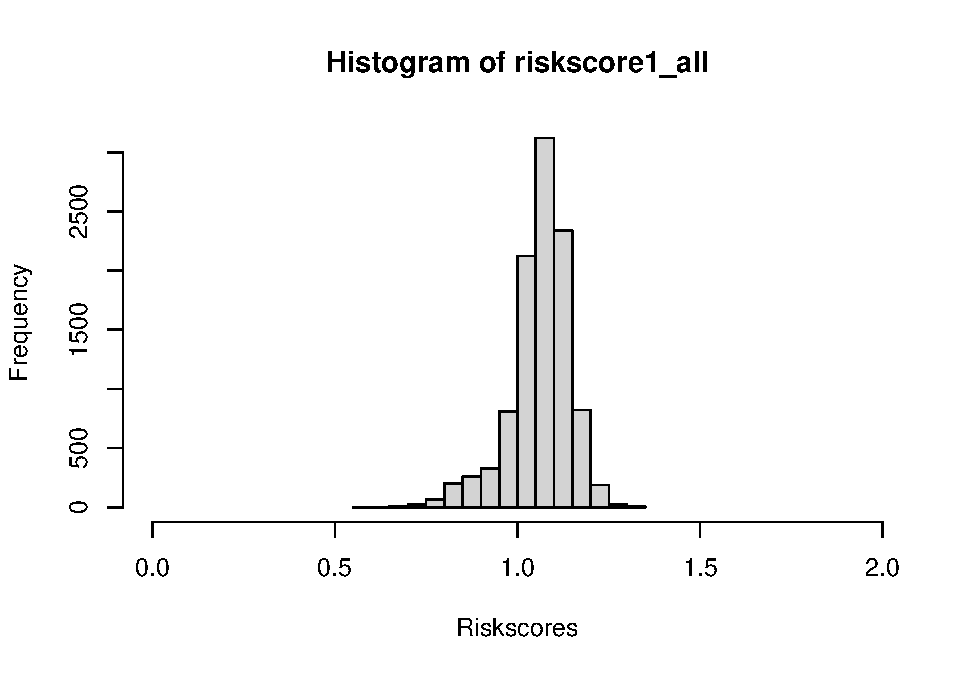
\includegraphics{Hazard_and_Risk_plot_updated_files/figure-latex/unnamed-chunk-6-1.pdf}

\begin{Shaded}
\begin{Highlighting}[]
\CommentTok{\#Density plot of riskscores}
\CommentTok{\# TRAIN\_RISK \textless{}{-} data.frame(rs=riskscore1\_train)}
\CommentTok{\# TEST\_RISK \textless{}{-} data.frame(rs=riskscore1\_test)}
\NormalTok{ALL\_DATA }\OtherTok{\textless{}{-}} \FunctionTok{data.frame}\NormalTok{(}\AttributeTok{Riskscores=}\NormalTok{riskscore1\_all)}

\CommentTok{\# TRAIN\_RISK$type\textless{}{-}\textquotesingle{}train\textquotesingle{}}
\CommentTok{\# TEST\_RISK$type\textless{}{-}\textquotesingle{}test\textquotesingle{}}
\NormalTok{ALL\_DATA}\SpecialCharTok{$}\NormalTok{data}\OtherTok{\textless{}{-}}\StringTok{\textquotesingle{}Full Data\textquotesingle{}}
\FunctionTok{ggplot}\NormalTok{(ALL\_DATA, }\FunctionTok{aes}\NormalTok{(Riskscores, }\AttributeTok{fill=}\NormalTok{data)) }\SpecialCharTok{+} \FunctionTok{geom\_density}\NormalTok{(}\AttributeTok{alpha =} \FloatTok{0.5}\NormalTok{) }
\end{Highlighting}
\end{Shaded}

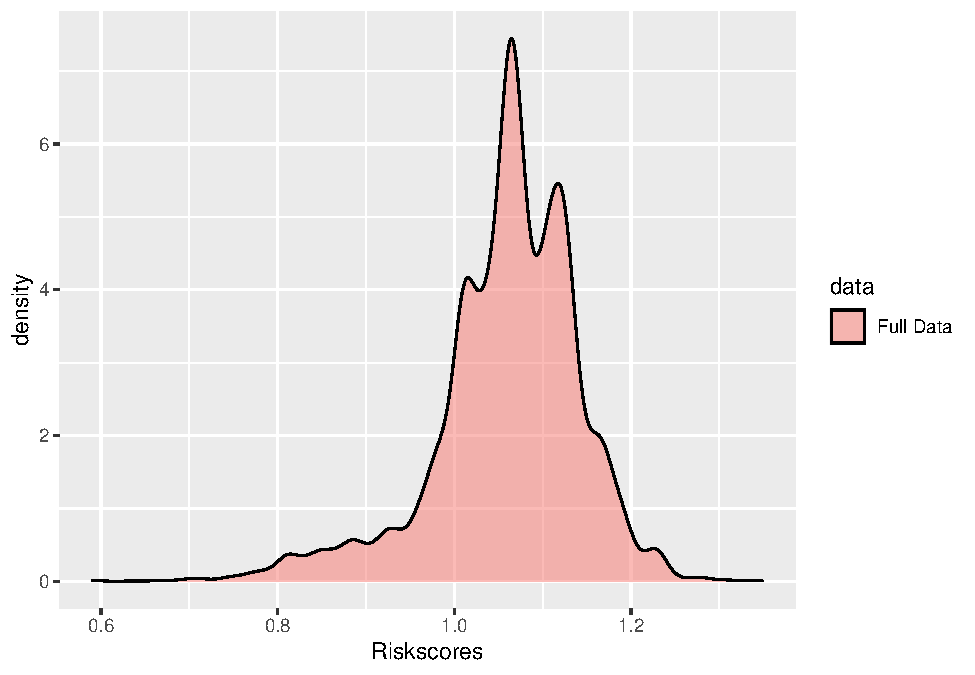
\includegraphics{Hazard_and_Risk_plot_updated_files/figure-latex/unnamed-chunk-6-2.pdf}

\begin{Shaded}
\begin{Highlighting}[]
\CommentTok{\# ggplot(TEST\_RISK, aes(rs, fill=type)) + geom\_density(alpha = 0.2) }
\CommentTok{\# ggplot(TRAIN\_RISK, aes(rs, fill=type)) + geom\_density(alpha = 0.2) }
\CommentTok{\# }
\CommentTok{\# datlen\textless{}{-}rbind(TRAIN\_RISK,TEST\_RISK,ALL\_DATA)}
\CommentTok{\# ggplot(datlen, aes(rs, fill=type)) + geom\_density(alpha = 0.2)}
\end{Highlighting}
\end{Shaded}

\newpage
\section{Hazard Ratios}

\begin{Shaded}
\begin{Highlighting}[]
\NormalTok{lphr3}\OtherTok{=}\FunctionTok{predict}\NormalTok{(cox\_fit1, }\AttributeTok{type=}\StringTok{"lp"}\NormalTok{) }\CommentTok{\#predicted hazard ratio}

\CommentTok{\# hist(lphr3, xlim = c(0,2), xlab = "HR")}
\CommentTok{\# hist(1{-}lphr3, xlim = c(0,2), xlab = "HR")}
\FunctionTok{range}\NormalTok{(lphr3)}
\end{Highlighting}
\end{Shaded}

\begin{verbatim}
## [1] -0.526645  0.298877
\end{verbatim}

\begin{Shaded}
\begin{Highlighting}[]
\FunctionTok{range}\NormalTok{(}\DecValTok{1}\SpecialCharTok{{-}}\NormalTok{lphr3)}
\end{Highlighting}
\end{Shaded}

\begin{verbatim}
## [1] 0.701123 1.526645
\end{verbatim}

\begin{Shaded}
\begin{Highlighting}[]
\NormalTok{ALLDATA }\OtherTok{\textless{}{-}} \FunctionTok{data.frame}\NormalTok{(}\AttributeTok{Hazard\_Ratios=}\NormalTok{lphr3)}
\NormalTok{ALLDATA}\SpecialCharTok{$}\NormalTok{data}\OtherTok{\textless{}{-}}\StringTok{\textquotesingle{}Full Data\textquotesingle{}}
\FunctionTok{ggplot}\NormalTok{(ALLDATA, }\FunctionTok{aes}\NormalTok{(Hazard\_Ratios, }\AttributeTok{fill=}\NormalTok{data)) }\SpecialCharTok{+} \FunctionTok{geom\_density}\NormalTok{(}\AttributeTok{alpha =} \FloatTok{0.5}\NormalTok{) }
\end{Highlighting}
\end{Shaded}

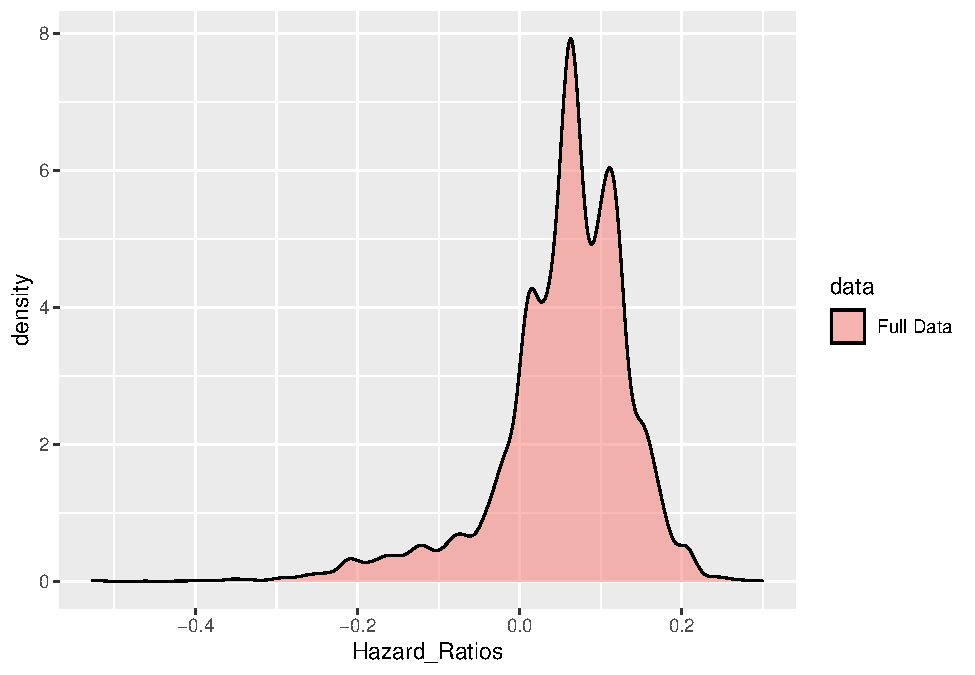
\includegraphics{Hazard_and_Risk_plot_updated_files/figure-latex/unnamed-chunk-7-1.pdf}

\begin{Shaded}
\begin{Highlighting}[]
\NormalTok{ALLDATA }\OtherTok{\textless{}{-}} \FunctionTok{data.frame}\NormalTok{(}\AttributeTok{Hazard\_Ratios1=}\DecValTok{1}\SpecialCharTok{{-}}\NormalTok{lphr3)}
\NormalTok{ALLDATA}\SpecialCharTok{$}\NormalTok{data}\OtherTok{\textless{}{-}}\StringTok{\textquotesingle{}Full Data\textquotesingle{}}
\FunctionTok{ggplot}\NormalTok{(ALLDATA, }\FunctionTok{aes}\NormalTok{(Hazard\_Ratios1, }\AttributeTok{fill=}\NormalTok{data)) }\SpecialCharTok{+} \FunctionTok{geom\_density}\NormalTok{(}\AttributeTok{alpha =} \FloatTok{0.5}\NormalTok{)}
\end{Highlighting}
\end{Shaded}

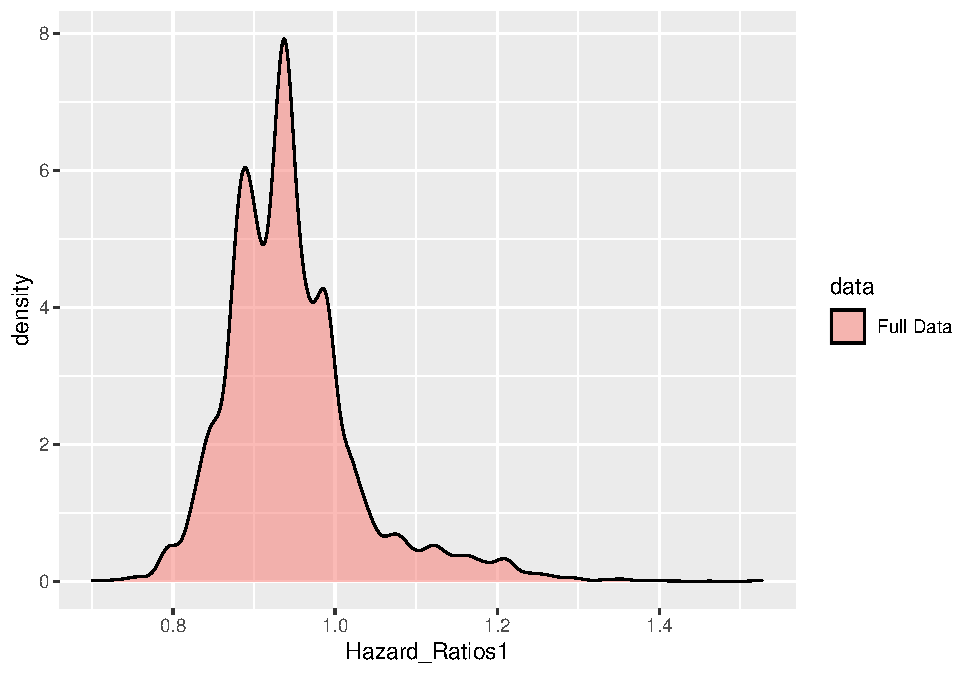
\includegraphics{Hazard_and_Risk_plot_updated_files/figure-latex/unnamed-chunk-7-2.pdf}

\newpage
\section{Scatterplots of Riskscores vs Hazard Ratios}

\begin{Shaded}
\begin{Highlighting}[]
\FunctionTok{plot}\NormalTok{(riskscore1\_all, lphr3, }\AttributeTok{ylab =} \StringTok{"Hazard Ratio"}\NormalTok{ ,}
     \AttributeTok{xlab=}\StringTok{"risk score"}\NormalTok{, }\AttributeTok{col=}\StringTok{"blue"}\NormalTok{)}
\NormalTok{v}\OtherTok{=}\FunctionTok{quantile}\NormalTok{(riskscore1\_all)}
\FunctionTok{abline}\NormalTok{(}\AttributeTok{h=}\DecValTok{0}\NormalTok{, }\AttributeTok{lty=}\DecValTok{2}\NormalTok{, }\AttributeTok{lwd=}\DecValTok{2}\NormalTok{, }\AttributeTok{col=}\StringTok{"red"}\NormalTok{)}
\FunctionTok{abline}\NormalTok{(}\AttributeTok{v=}\DecValTok{1}\NormalTok{, }\AttributeTok{lwd=}\DecValTok{3}\NormalTok{, }\AttributeTok{col=}\StringTok{"red"}\NormalTok{)}
\FunctionTok{abline}\NormalTok{(}\AttributeTok{v=}\NormalTok{v[}\DecValTok{2}\NormalTok{], }\AttributeTok{lwd=}\DecValTok{3}\NormalTok{, }\AttributeTok{col=}\StringTok{"snow3"}\NormalTok{)}
\FunctionTok{abline}\NormalTok{(}\AttributeTok{v=}\NormalTok{v[}\DecValTok{1}\NormalTok{], }\AttributeTok{lwd=}\DecValTok{3}\NormalTok{, }\AttributeTok{col=}\StringTok{"snow3"}\NormalTok{)}
\FunctionTok{abline}\NormalTok{(}\AttributeTok{v=}\NormalTok{v[}\DecValTok{3}\NormalTok{], }\AttributeTok{lwd=}\DecValTok{3}\NormalTok{, }\AttributeTok{col=}\StringTok{"snow3"}\NormalTok{)}
\FunctionTok{abline}\NormalTok{(}\AttributeTok{v=}\NormalTok{v[}\DecValTok{4}\NormalTok{], }\AttributeTok{lwd=}\DecValTok{3}\NormalTok{, }\AttributeTok{col=}\StringTok{"snow3"}\NormalTok{)}
\end{Highlighting}
\end{Shaded}

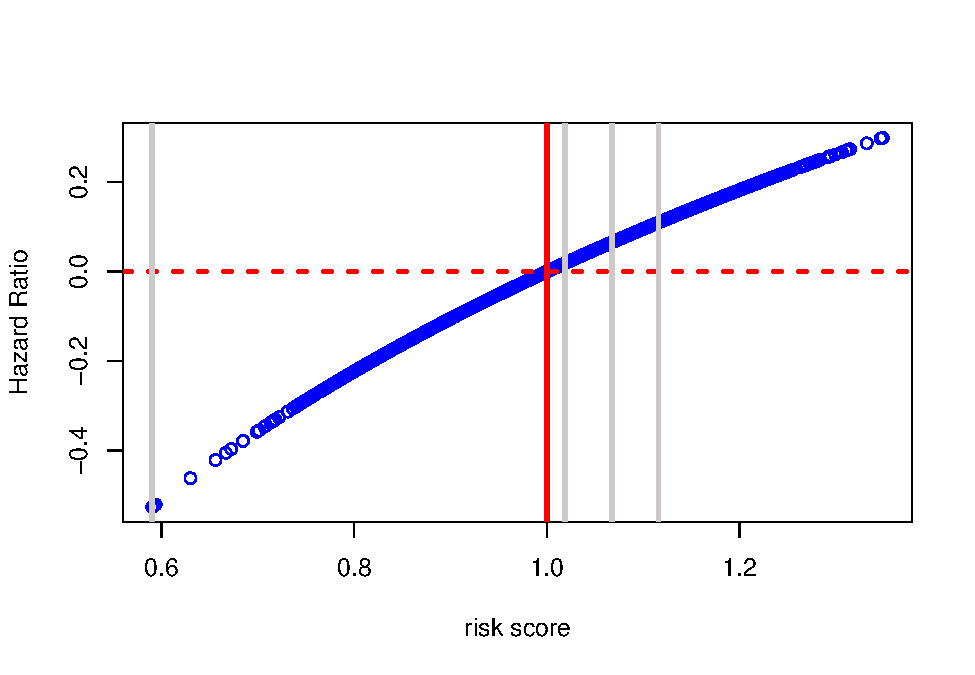
\includegraphics{Hazard_and_Risk_plot_updated_files/figure-latex/unnamed-chunk-8-1.pdf}
\textbf{Comment} \newline \textbf{\emph{A positive HR indicates worse
conditions/prognosis, while a negative coefficient indicates a better
condition/prognosis.}}\newline Riskscores \textgreater{} 1 corresponds
to increased hazards of mortality with multiple HRF. Riskscores
\textless{} 1 corresponds to decreased hazards of mortality with
multiple HRF, thus a survival benefit from chemotherapy.\newline  The
threshold for survival benefit is experienced when the risk score is
\textless{} 1 at which point the hazards of mortality is decreased.

\newpage

\begin{Shaded}
\begin{Highlighting}[]
\FunctionTok{plot}\NormalTok{(riskscore1\_all, }\DecValTok{1}\SpecialCharTok{{-}}\NormalTok{lphr3, }\AttributeTok{ylab =} \StringTok{"Hazard Ratio"}\NormalTok{, }\AttributeTok{xlab=}\StringTok{"Risk Score"}\NormalTok{,}
     \AttributeTok{main=} \StringTok{"Hazard Ratio vs RiskScores"}\NormalTok{,}\AttributeTok{col=}\StringTok{"blue"}\NormalTok{)}\CommentTok{\# ylim=c(0.6,1.6), xlim=c(0.6,1.6)}

\FunctionTok{abline}\NormalTok{(}\AttributeTok{h=}\DecValTok{1}\NormalTok{, }\AttributeTok{lty=}\DecValTok{2}\NormalTok{, }\AttributeTok{lwd=}\DecValTok{2}\NormalTok{, }\AttributeTok{col=}\StringTok{"red"}\NormalTok{)}
\FunctionTok{abline}\NormalTok{(}\AttributeTok{v=}\DecValTok{1}\NormalTok{, }\AttributeTok{lwd=}\DecValTok{3}\NormalTok{, }\AttributeTok{col=}\StringTok{"red"}\NormalTok{)}
\FunctionTok{abline}\NormalTok{(}\AttributeTok{v=}\NormalTok{v[}\DecValTok{2}\NormalTok{], }\AttributeTok{lwd=}\DecValTok{3}\NormalTok{, }\AttributeTok{col=}\StringTok{"snow3"}\NormalTok{)}
\FunctionTok{abline}\NormalTok{(}\AttributeTok{v=}\NormalTok{v[}\DecValTok{1}\NormalTok{], }\AttributeTok{lwd=}\DecValTok{3}\NormalTok{, }\AttributeTok{col=}\StringTok{"snow3"}\NormalTok{)}
\FunctionTok{abline}\NormalTok{(}\AttributeTok{v=}\NormalTok{v[}\DecValTok{3}\NormalTok{], }\AttributeTok{lwd=}\DecValTok{3}\NormalTok{, }\AttributeTok{col=}\StringTok{"snow3"}\NormalTok{)}
\FunctionTok{abline}\NormalTok{(}\AttributeTok{v=}\NormalTok{v[}\DecValTok{4}\NormalTok{], }\AttributeTok{lwd=}\DecValTok{3}\NormalTok{, }\AttributeTok{col=}\StringTok{"snow3"}\NormalTok{)}
\end{Highlighting}
\end{Shaded}

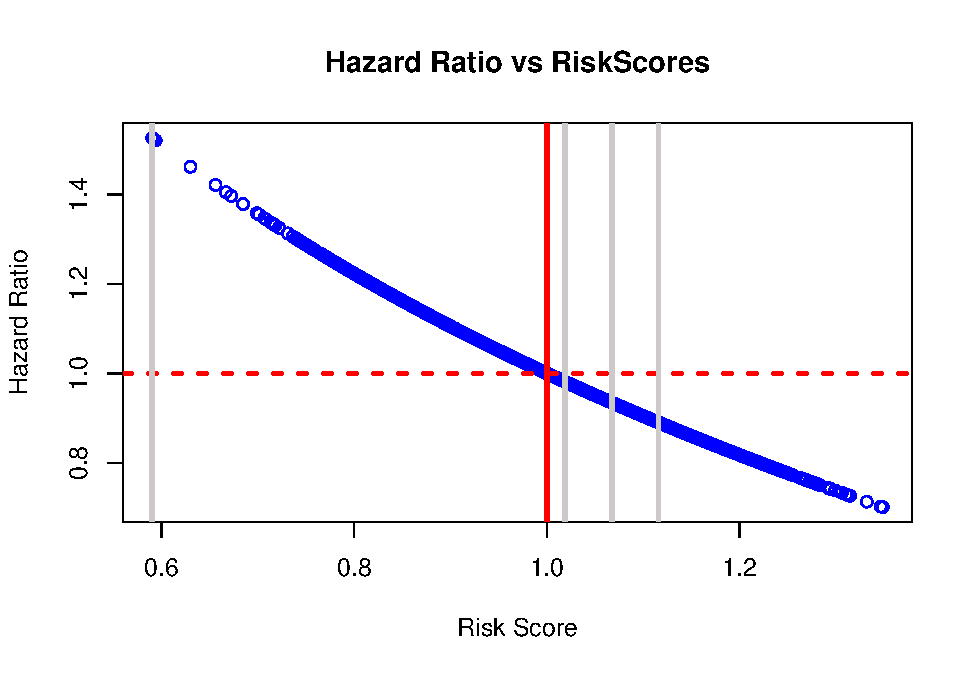
\includegraphics{Hazard_and_Risk_plot_updated_files/figure-latex/unnamed-chunk-9-1.pdf}
\textbf{\emph{Subtracting HR from 1 gives reverse scale of HR reads,
where lower HR indicates worse conditions, higher HR indicates better
prognosis}}\newline As risk score increases, the hazard ratio gets worse
(bad prognosis). A survival benefit from adjuvant chemotherapy is
realised when the risk score is \textless{} 1 at which point the hazard
ratio of mortality appears to be better.\newline  \textbf{\emph{Note the
reverse reading of the Hazard ratio scale.}}

\begin{center}\rule{0.5\linewidth}{0.5pt}\end{center}

\newpage
\section{Riskscores from Est.PH}

\hypertarget{est.ph-survc1---derivation-of-a-risk-score-by-a-cox-proportioal-hazard-model}{%
\section{Est.PH \{survC1\} - Derivation of a risk score by a Cox
proportioal hazard
model}\label{est.ph-survc1---derivation-of-a-risk-score-by-a-cox-proportioal-hazard-model}}

\hypertarget{obtain-risk-scores-from-the-best-predictors-of-mortality}{%
\subsection{Obtain Risk scores from the best predictors of
mortality}\label{obtain-risk-scores-from-the-best-predictors-of-mortality}}

\begin{Shaded}
\begin{Highlighting}[]
\CommentTok{\#Provides risk score by fitting data to a Cox\textquotesingle{}s proportional hazards model with a given set of predictors}
\CommentTok{\# Input data. The 1st column should be time{-}to{-}event, and the 2nd column is event indicator (1=event, 0=censor). The rest of the columns are covariates/predictors used in the model. No character variable or missing is allowed. }
\CommentTok{\#OUTPUT}
\CommentTok{\# beta = Estimates for regression coefficient in the Cox model}
\CommentTok{\# var = Variance{-}Covariance matrix for the beta above}
\CommentTok{\# rs    = Risk score of each individual}
\CommentTok{\# ft    = coxph object with the fitted model}

\FunctionTok{library}\NormalTok{(survC1)}
\end{Highlighting}
\end{Shaded}

\begin{verbatim}
## Warning: package 'survC1' was built under R version 4.0.5
\end{verbatim}

\begin{Shaded}
\begin{Highlighting}[]
\NormalTok{train1}\OtherTok{=}\NormalTok{lung[,}\FunctionTok{c}\NormalTok{(}\DecValTok{1}\SpecialCharTok{:}\DecValTok{2}\NormalTok{)] }\CommentTok{\#time \& status}

\NormalTok{train2 }\OtherTok{=}\NormalTok{lung[, }\FunctionTok{c}\NormalTok{(}\DecValTok{3}\SpecialCharTok{:}\DecValTok{15}\NormalTok{)] }\CommentTok{\# other covariates}

\CommentTok{\#convert other sub levels in all categorical covariates to integer}
\NormalTok{p }\OtherTok{=} \FunctionTok{data.frame}\NormalTok{(}\FunctionTok{lapply}\NormalTok{(train2, as.integer))}

\CommentTok{\#combine numeric time \& status with the numeric covariates}
\NormalTok{train\_data }\OtherTok{=} \FunctionTok{data.frame}\NormalTok{(}\FunctionTok{cbind}\NormalTok{(train1,p)) }

\CommentTok{\#Make sure distribution of variables are not distorted after conversion}
\FunctionTok{require}\NormalTok{(inspectdf)}
\end{Highlighting}
\end{Shaded}

\begin{verbatim}
## Loading required package: inspectdf
\end{verbatim}

\begin{verbatim}
## Warning: package 'inspectdf' was built under R version 4.0.5
\end{verbatim}

\begin{Shaded}
\begin{Highlighting}[]
\FunctionTok{show\_plot}\NormalTok{(}\FunctionTok{inspect\_cat}\NormalTok{(train)) }\CommentTok{\# inspect categorical columns }
\end{Highlighting}
\end{Shaded}

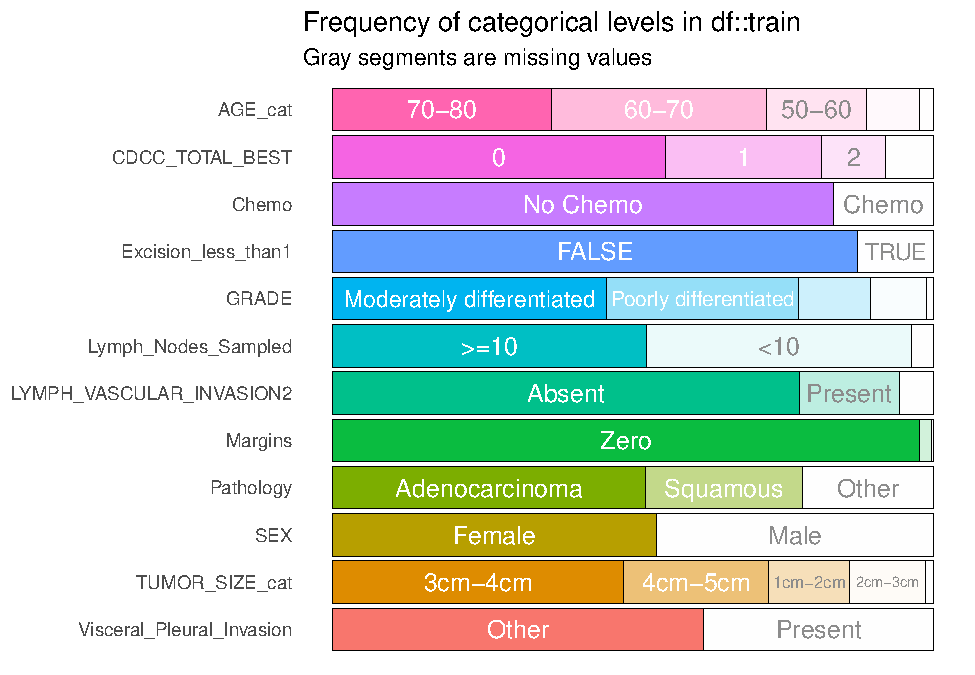
\includegraphics{Hazard_and_Risk_plot_updated_files/figure-latex/unnamed-chunk-10-1.pdf}

\begin{Shaded}
\begin{Highlighting}[]
\FunctionTok{show\_plot}\NormalTok{(}\FunctionTok{inspect\_num}\NormalTok{(train)) }\CommentTok{\#inspect numeric columns }
\end{Highlighting}
\end{Shaded}

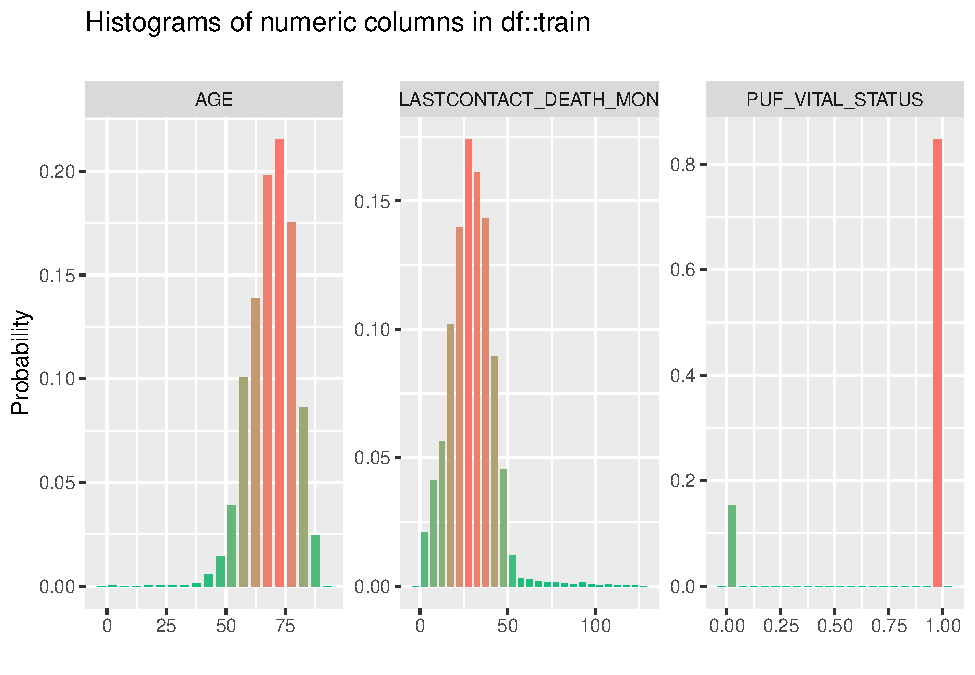
\includegraphics{Hazard_and_Risk_plot_updated_files/figure-latex/unnamed-chunk-10-2.pdf}

\begin{Shaded}
\begin{Highlighting}[]
\FunctionTok{show\_plot}\NormalTok{(}\FunctionTok{inspect\_num}\NormalTok{(train\_data)) }\CommentTok{\#inspect numeric columns }
\end{Highlighting}
\end{Shaded}

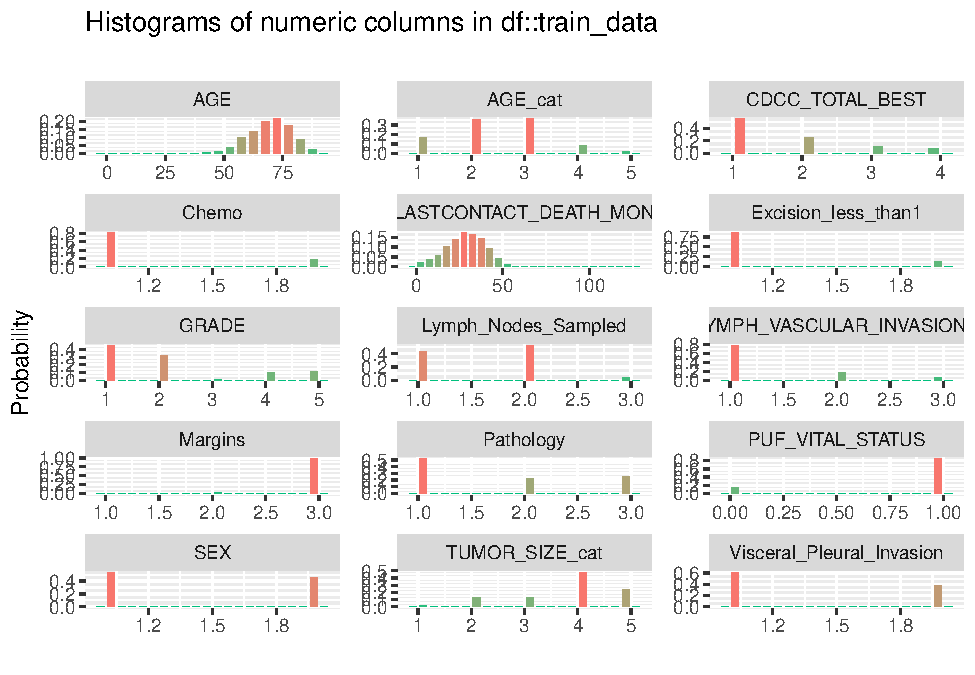
\includegraphics{Hazard_and_Risk_plot_updated_files/figure-latex/unnamed-chunk-10-3.pdf}

\begin{Shaded}
\begin{Highlighting}[]
\CommentTok{\#obtain risk scores for each individual}
\NormalTok{rsmodel}\OtherTok{=}\FunctionTok{Est.PH}\NormalTok{(train\_data)}
\NormalTok{riskscores}\OtherTok{=}\NormalTok{rsmodel}\SpecialCharTok{$}\NormalTok{rs}
\FunctionTok{hist}\NormalTok{(riskscores)}
\end{Highlighting}
\end{Shaded}

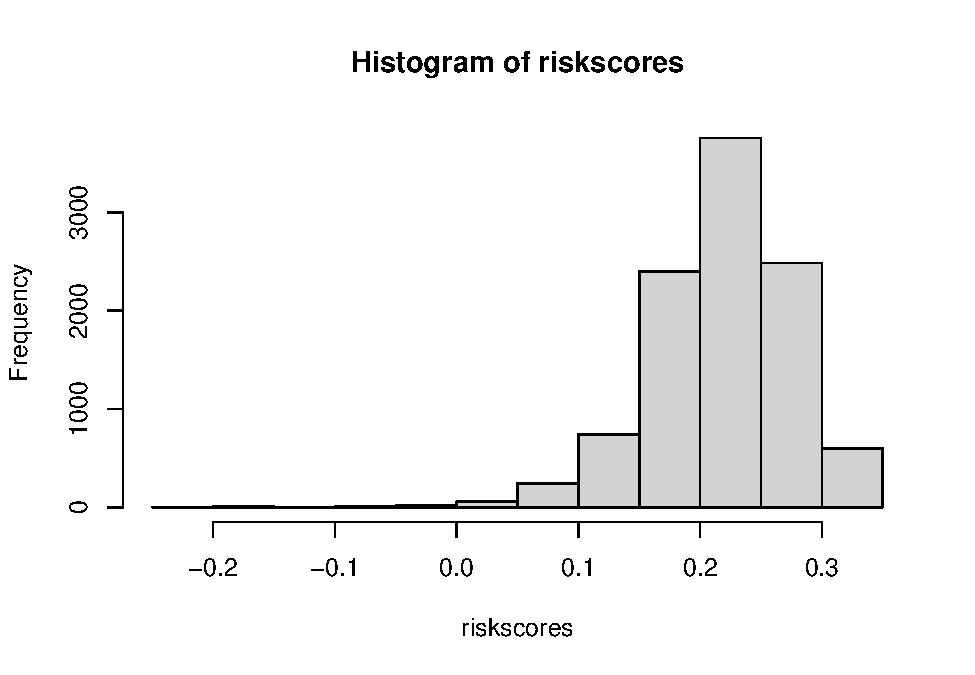
\includegraphics{Hazard_and_Risk_plot_updated_files/figure-latex/unnamed-chunk-11-1.pdf}

\begin{Shaded}
\begin{Highlighting}[]
\FunctionTok{hist}\NormalTok{(}\DecValTok{1}\SpecialCharTok{{-}}\NormalTok{riskscores)}
\end{Highlighting}
\end{Shaded}

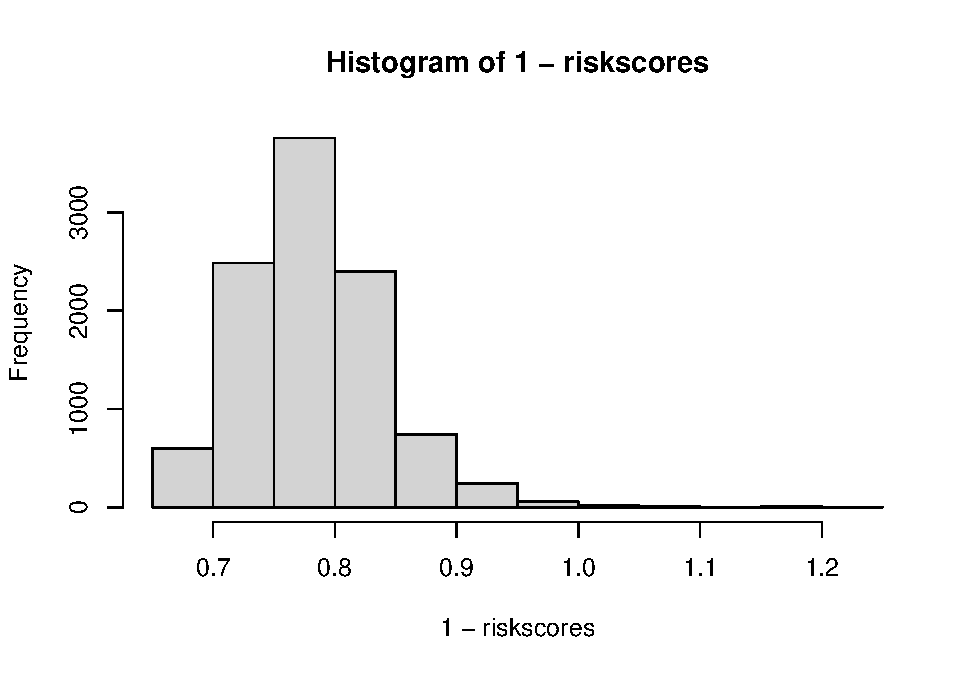
\includegraphics{Hazard_and_Risk_plot_updated_files/figure-latex/unnamed-chunk-11-2.pdf}

\begin{Shaded}
\begin{Highlighting}[]
\CommentTok{\#riskscores1 = 1 {-} riskscores}
\end{Highlighting}
\end{Shaded}

\begin{Shaded}
\begin{Highlighting}[]
\CommentTok{\#obtain hazard rates .... didnt work with this approach}
\NormalTok{coef}\OtherTok{=}\NormalTok{rsmodel}\SpecialCharTok{$}\NormalTok{beta}
\FunctionTok{exp}\NormalTok{(coef)}
\end{Highlighting}
\end{Shaded}

\begin{verbatim}
##                     covsChemo                       covsAGE 
##                     0.9772929                     1.0010946 
##                   covsAGE_cat                       covsSEX 
##                     0.9791978                     0.9486315 
##           covsCDCC_TOTAL_BEST            covsTUMOR_SIZE_cat 
##                     1.0025016                     1.0005138 
##                     covsGRADE                 covsPathology 
##                     0.9915676                     1.0041478 
## covsVisceral_Pleural_Invasion  covsLYMPH_VASCULAR_INVASION2 
##                     1.0490644                     0.9495022 
##                   covsMargins       covsLymph_Nodes_Sampled 
##                     1.1256563                     0.9935250 
##       covsExcision_less_than1 
##                     0.9654898
\end{verbatim}

\begin{Shaded}
\begin{Highlighting}[]
\FunctionTok{hist}\NormalTok{(}\FunctionTok{sqrt}\NormalTok{(riskscores))}
\end{Highlighting}
\end{Shaded}

\begin{verbatim}
## Warning in sqrt(riskscores): NaNs produced
\end{verbatim}

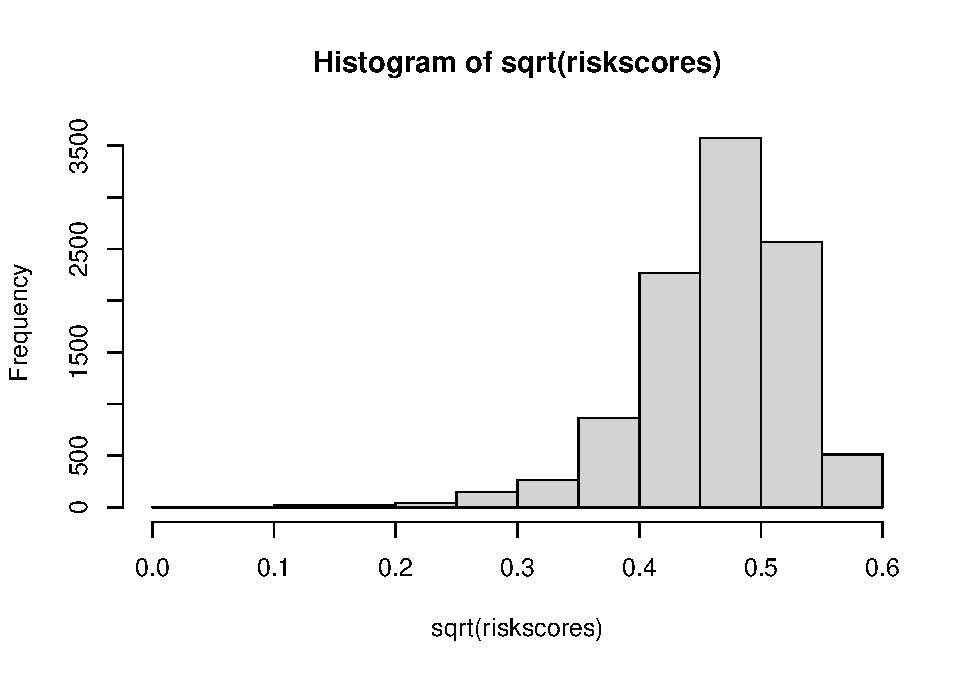
\includegraphics{Hazard_and_Risk_plot_updated_files/figure-latex/unnamed-chunk-12-1.pdf}

\begin{Shaded}
\begin{Highlighting}[]
\CommentTok{\#riskscores1 = 1 {-} riskscores}
\end{Highlighting}
\end{Shaded}

\begin{Shaded}
\begin{Highlighting}[]
\CommentTok{\# lphr3=predict(cox\_fit3, lung, type="lp") \#predicted hazard ratio}
\CommentTok{\# hrrr=1{-}lphr3}
\end{Highlighting}
\end{Shaded}

\begin{Shaded}
\begin{Highlighting}[]
\FunctionTok{plot}\NormalTok{(riskscores, }\DecValTok{1}\SpecialCharTok{{-}}\NormalTok{lphr3, }\AttributeTok{ylab =} \StringTok{"Hazard Ratio"}\NormalTok{ ,}
     \AttributeTok{xlab=}\StringTok{"Risk Score"}\NormalTok{, }\AttributeTok{col=}\StringTok{"blue"}\NormalTok{)}\CommentTok{\# ylim=c(0.6,1.6), xlim=c(0.6,1.6)}

\FunctionTok{abline}\NormalTok{(}\AttributeTok{h=}\DecValTok{1}\NormalTok{, }\AttributeTok{lty=}\DecValTok{2}\NormalTok{, }\AttributeTok{lwd=}\DecValTok{2}\NormalTok{, }\AttributeTok{col=}\StringTok{"red"}\NormalTok{)}
\FunctionTok{abline}\NormalTok{(}\AttributeTok{v=}\DecValTok{1}\NormalTok{, }\AttributeTok{lwd=}\DecValTok{3}\NormalTok{, }\AttributeTok{col=}\StringTok{"red"}\NormalTok{)}
\FunctionTok{abline}\NormalTok{(}\AttributeTok{v=}\NormalTok{v[}\DecValTok{2}\NormalTok{], }\AttributeTok{lwd=}\DecValTok{3}\NormalTok{, }\AttributeTok{col=}\StringTok{"snow3"}\NormalTok{)}
\FunctionTok{abline}\NormalTok{(}\AttributeTok{v=}\NormalTok{v[}\DecValTok{1}\NormalTok{], }\AttributeTok{lwd=}\DecValTok{3}\NormalTok{, }\AttributeTok{col=}\StringTok{"snow3"}\NormalTok{)}
\FunctionTok{abline}\NormalTok{(}\AttributeTok{v=}\NormalTok{v[}\DecValTok{3}\NormalTok{], }\AttributeTok{lwd=}\DecValTok{3}\NormalTok{, }\AttributeTok{col=}\StringTok{"snow3"}\NormalTok{)}
\FunctionTok{abline}\NormalTok{(}\AttributeTok{v=}\NormalTok{v[}\DecValTok{4}\NormalTok{], }\AttributeTok{lwd=}\DecValTok{3}\NormalTok{, }\AttributeTok{col=}\StringTok{"snow3"}\NormalTok{)}
\end{Highlighting}
\end{Shaded}

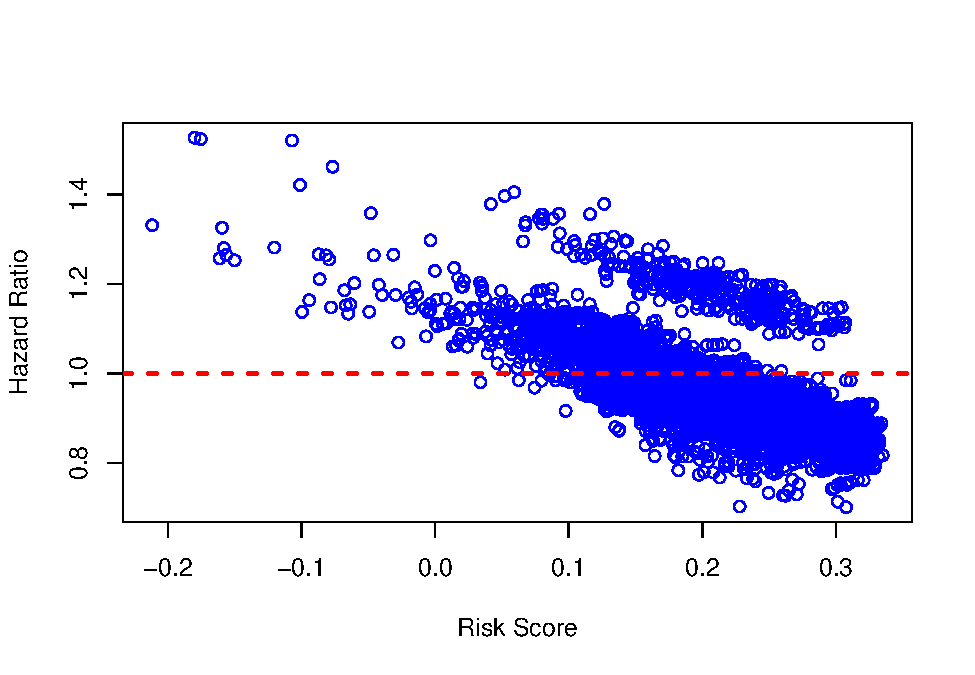
\includegraphics{Hazard_and_Risk_plot_updated_files/figure-latex/unnamed-chunk-14-1.pdf}

\end{document}
